% Review 2 report: forecasting daily mean temperature at eight NOAA GSOD stations.
% Compile: tectonic review_2_report.tex   (or xelatex/pdflatex -> bibtex -> x2)
\documentclass[11pt,a4paper]{article}

% ---- Course details: fill these in; empty fields are omitted from the title page.
\newcommand*{\CourseName}{}
\newcommand*{\Institution}{}
\newcommand*{\Instructor}{}

\usepackage[a4paper,margin=2.4cm,headheight=14pt]{geometry}
\usepackage{iftex}
\ifTUTeX
  \usepackage{fontspec}% XeLaTeX/LuaLaTeX (Tectonic): Latin Modern via OpenType
\else
  \usepackage[T1]{fontenc}
  \usepackage{lmodern}
\fi
\usepackage{microtype}
\usepackage{amsmath,amssymb,bm}
\usepackage{siunitx}
\sisetup{detect-all}
\usepackage{graphicx}
\usepackage{booktabs}
\usepackage{tabularx}
\usepackage{caption}
\usepackage{subcaption}
\usepackage{float}
\usepackage{enumitem}
\usepackage{xcolor}
\usepackage{fancyhdr}
\usepackage[round,authoryear]{natbib}
\usepackage[hidelinks]{hyperref}
\usepackage{xurl}
\usepackage[capitalise,noabbrev]{cleveref}

\graphicspath{{figures/}}
\captionsetup{font=small,labelfont=bf,margin=0.5cm}
\setlist{itemsep=2pt,topsep=4pt}
\newcommand{\degC}{\,\si{\degreeCelsius}}
\newcommand{\code}[1]{\texttt{#1}}
\renewcommand{\arraystretch}{1.12}
\makeatletter
\newcommand{\tabfile}[1]{\@@input #1 }
\makeatother
\newcolumntype{L}{>{\raggedright\arraybackslash}X}

\pagestyle{fancy}
\fancyhf{}
\lhead{\small NOAA GSOD time-series case study}
\rhead{\small Review 2}
\cfoot{\small\thepage}

\title{\textbf{Forecasting Daily Mean Temperature at Eight Indian Weather Stations}\\[4pt]
\large Statistical, Machine-Learning and Deep-Learning Models on NOAA GSOD Data, 2010--2024\\[2pt]
\normalsize Review 2 report}
\author{Kushal Yalamanchi \and Kushaal K N \and Dhrusheek}
\date{%
  \ifx\CourseName\empty\else\CourseName\\\fi
  \ifx\Institution\empty\else\Institution\\\fi
  \ifx\Instructor\empty\else Instructor: \Instructor\\\fi
  October 2026}

\begin{document}
\maketitle
\thispagestyle{fancy}

\begin{abstract}
\noindent
We compare fourteen one-day-ahead forecasting methods for daily mean temperature at eight NOAA GSOD stations (Bengaluru, Delhi, Mumbai, Chennai, Kolkata, Hyderabad, Ahmedabad, Pune), all scored on the same 822-day test period from 2 October 2022 to 31 December 2024. The methods are four naive baselines, ARIMA, SARIMA, ARMAX and SARIMAX with orders chosen per city by BIC, two Holt--Winters variants, random forest, gradient boosting, an LSTM and a Transformer. Linear ARMA models with annual and weekly Fourier regressors (ARMAX and SARIMAX) give the lowest mean RMSE across cities (1.016\degC, 5.2\% below persistence) and the lowest RMSE in five cities; tree ensembles win the other three. The seven best methods are separated by only 0.022\degC{} in mean RMSE, however. After Holm correction, a Diebold--Mariano test finds the best model significantly better than persistence in absolute loss only for Ahmedabad, Delhi and Chennai. Forecast difficulty differs far more between cities than between models. The best RMSE ranges from 0.826\degC{} (Bengaluru) to 1.338\degC{} (Delhi) and follows the typical size of day-to-day temperature change (Spearman $\rho = 0.90$, $n = 8$). At leads of up to 30 days, a direct multi-output Transformer reduces mean MAE by 11.8--30.6\% relative to persistence and by 16.0--27.0\% relative to a seasonal naive forecast, although no significance test was run at these horizons. Residuals of the selected models are non-Gaussian with heavier cold-side tails everywhere and keep small but detectable autocorrelation in five cities.
\end{abstract}

\section{Introduction}
\label{sec:intro}

Our Review 1 report characterised daily mean temperature at the eight stations used here. Every series was stationary around a strong annual cycle (STL seasonal strength 0.64--0.93), had a lag-1 autocorrelation of 0.90--0.98 and a partial autocorrelation dominated by lag 1, and showed no consistent trend. The cities differed mainly in seasonal amplitude (5.3--20.7\degC) and in the average size of day-to-day changes (0.62--1.13\degC). Review 1 ended with three hypotheses:
\begin{description}[style=nextline,leftmargin=1.2em]
  \item[H1] Models that use recent history will clearly beat mean and seasonal-naive baselines and can match or improve on persistence one day ahead.
  \item[H0] Learned sequence structure gives no material improvement over persistence one day ahead.
  \item[H2] Across cities, one-day-ahead error will follow day-to-day variability more closely than seasonal strength, and the gain of any model over persistence will be small at one day and larger at longer leads.
\end{description}

This report tests them. We ask three questions. Which model families forecast next-day temperature best under an identical protocol, and by how much do they beat persistence? Do those gains hold up under paired significance testing and residual diagnostics? And why are some cities so much harder to forecast than others? \Cref{sec:protocol} describes the data split and the two analysis pipelines, \cref{sec:models} the models and how ARIMA orders were chosen, and \cref{sec:eval} the metrics and tests. Results follow in \cref{sec:results}, and \cref{sec:discussion,sec:limits} interpret them and set out their limits.

\section{Data and experimental protocol}
\label{sec:protocol}

\subsection{Data}

The data are daily mean temperatures from NOAA NCEI's \emph{Global Surface Summary of the Day} \citep{ncei_gsod}, downloaded per station and year from
\begin{center}
\small\url{https://www.ncei.noaa.gov/data/global-summary-of-the-day/access/}\quad(file pattern \code{\{YEAR\}/\{STATION\}.csv}).
\end{center}
\Cref{tab:stations} lists the stations. Each series covers 1 January 2010 to 31 December 2024 on a continuous calendar of $n = 5{,}479$ days. Temperatures were converted from \textdegree F to \textdegree C, and the 12--66 missing days per station (at most 1.2\%) were filled by linear time interpolation; Review 1 (Section~3) documents the cleaning in full. Precipitation is not used: after correct handling of the GSOD \code{I} flag it is 47--77\% missing.

\begin{table}[ht]
\centering
\footnotesize
\caption{Stations (GSOD identifiers are USAF+WBAN). Elevations from the GSOD files.}
\label{tab:stations}
\begin{tabular}{@{}l l l r@{}}
\toprule
City & GSOD station & Station name & Elev.\ (m) \\
\midrule
Bengaluru & \code{43295099999} & Bangalore & 921 \\
Delhi & \code{42182099999} & Safdarjung & 215 \\
Mumbai & \code{43003099999} & Chhatrapati Shivaji International & 11 \\
Chennai & \code{43279099999} & Chennai International & 16 \\
Kolkata & \code{42809099999} & Netaji Subhash Chandra Bose International & 5 \\
Hyderabad & \code{43128099999} & Begumpet Airport & 531 \\
Ahmedabad & \code{42647099999} & Ahmedabad & 58 \\
Pune & \code{43063099999} & Pune & 558 \\
\bottomrule
\end{tabular}
\end{table}

\subsection{Chronological split}

Every series is divided at the same positions, without shuffling:
\begin{center}
\small
\begin{tabular}{@{}l l r@{}}
\toprule
Segment & Dates & Days \\
\midrule
Training & 2010-01-01 to 2020-07-01 & 3{,}835 \\
Validation & 2020-07-02 to 2022-10-01 & 822 \\
Test & 2022-10-02 to 2024-12-31 & 822 \\
\bottomrule
\end{tabular}
\end{center}
The test segment is identical across cities, so all cities are scored on the same days and the same seasons. It was used only to compute the reported scores: no order, hyperparameter or stopping epoch was chosen on it.

\subsection{Two pipelines}

The results come from two scripts that share the data, split, seeds and test dates.
\begin{itemize}
  \item \textbf{Stage A} (\nolinkurl{src/run_all_cities.py}) fits the naive baselines, an ARIMA(2,0,2) of fixed order, and the LSTM and Transformer. It is the only pipeline with a multi-horizon experiment (direct forecasts up to 30 days).
  \item \textbf{Stage B} (\nolinkurl{src/rubric_extension.py}) adds the per-city order selection for ARIMA, SARIMA, ARMAX and SARIMAX, two Holt--Winters models, random forest and gradient boosting, and retrains the LSTM and Transformer with the Stage A settings. It also runs the paired tests and residual diagnostics. All one-step rankings in this report come from Stage B.
\end{itemize}
The six models common to both pipelines (four naive baselines, LSTM, Transformer) give identical test MAE and RMSE in both result files at every city; the executed notebook checks this (Section~7.2). The two pipelines can therefore be read together.

\subsection{How each model family uses the data}

The families do not see the same amount of history, and this matters when comparing them (\cref{sec:limits}).
\begin{itemize}
  \item ARIMA-family and Holt--Winters models are estimated on training plus validation (4{,}657 days). Their parameters are then frozen, and the state is updated with each observed test value to produce one-step forecasts. Nothing is re-estimated during the test period.
  \item Tree ensembles are fitted on the same pre-test period (4{,}627 targets, since each needs 30 preceding days), with no use of the validation segment for tuning.
  \item LSTM and Transformer are fitted on the training segment only (3{,}805 input windows) and use the validation segment for early stopping. Inputs are standardised with the training mean and variance.
  \item The climatological-mean baseline uses the training mean, and MASE is scaled by the in-sample mean absolute daily change over the training segment.
\end{itemize}

\section{Models}
\label{sec:models}

Let $y_t$ be daily mean temperature and $\hat y_{t+h\mid t}$ a forecast made with information up to day $t$.

\subsection{Baselines}

Persistence forecasts $\hat y_{t+1\mid t} = y_t$; the seasonal naive forecasts are $\hat y_{t+1\mid t} = y_{t+1-m}$ with $m = 7$ and $m = 365$; and the climatological mean is the training-segment average. Review 1 showed that lag-1 autocorrelation is 0.90--0.98, so persistence is the benchmark that matters at one day ahead. We report skill relative to it,
\begin{equation}
  \mathrm{Skill}_{\mathrm{RMSE}} = 100\left(1 - \frac{\mathrm{RMSE}_{\text{model}}}{\mathrm{RMSE}_{\text{persistence}}}\right)\%,
  \label{eq:skill}
\end{equation}
and analogously for MAE \citep{murphy1988skill}.

\subsection{ARIMA-family models}

All four families are special cases of a regression with seasonal ARMA errors, fitted by maximum likelihood using the Kalman filter in the state-space implementation of \code{statsmodels} \citep{box2015time,seabold2010statsmodels}:
\begin{equation}
  \phi_p(B)\,\Phi_P(B^{7})\bigl(y_t - \bm\beta^{\top}\mathbf x_t\bigr) = c + \theta_q(B)\,\Theta_Q(B^{7})\,\varepsilon_t,
  \qquad \varepsilon_t \sim \mathrm{WN}(0,\sigma^2),
  \label{eq:sarimax}
\end{equation}
where $B$ is the backshift operator and $\phi_p$, $\theta_q$, $\Phi_P$, $\Theta_Q$ are polynomials of the indicated orders. ARIMA has no regressors and $P = Q = 0$. SARIMA adds weekly seasonal terms ($m = 7$). ARMAX and SARIMAX are the same two models with the regressor vector
\begin{equation}
  \mathbf x_t = \Bigl[\sin\tfrac{2\pi k\tau_t}{365.25},\; \cos\tfrac{2\pi k\tau_t}{365.25}\Bigr]_{k=1,2,3} \;\cup\; \Bigl[\sin\tfrac{2\pi t}{7},\; \cos\tfrac{2\pi t}{7}\Bigr],
  \label{eq:fourier}
\end{equation}
with $\tau_t$ the day of year minus one. Three annual harmonics give a smooth seasonal mean that can be asymmetric or double-peaked, as Mumbai's climatology is. These regressors are deterministic, so they are known in advance and introduce no information from future weather. One implementation detail departs from \cref{eq:fourier}: for ARMAX and SARIMAX the script computes the weekly terms from a day counter that restarts at zero for the test period, so the weekly phase shifts by two days at the train--test boundary ($4{,}657 \bmod 7 = 2$). The tree models use a continuous counter. Because the weekly terms carry very little information (\cref{sec:orders}), we expect the effect on accuracy to be small, but we did not measure it. A seasonal ARMA term with $m = 365$ would need lag polynomials of degree 365 and is impractical at daily resolution; the Fourier terms take its place.

\paragraph{Order selection.} The procedure in \code{src/rubric\_extension.py} uses only the 4{,}657 pre-test days of each city:
\begin{enumerate}
  \item \textbf{Differencing order $d$.} ADF and KPSS are applied to the level series; $d = 0$ is accepted if ADF rejects a unit root and KPSS does not reject stationarity, otherwise $d = 1$ is tried. All eight cities gave $d = 0$ (ADF $p \leq 0.0005$; KPSS $p \geq 0.08$), consistent with the full-series tests in Review 1. With no unit root, differencing would only introduce a non-invertible moving-average component.
  \item \textbf{Correlogram identification.} The ACF and PACF of the pre-test series and of its calendar-adjusted anomaly (the residual after regressing $y_t$ on $\mathbf x_t$) are shown in \cref{fig:acfpacf} and summarised in \cref{tab:orders}. The script also records an automatic hint, the largest of lags 1--3 whose ACF or PACF lies outside $\pm 1.96/\sqrt n$. Because all three lags were significant at every station, the hint equalled 3 everywhere and did not narrow the search; the grid below was fixed in advance.
  \item \textbf{Grid search.} All $(p,q) \in \{0,1,2\}^2$ are fitted. For SARIMA and SARIMAX, weekly seasonal variants $(P,Q) \in \{(0,1),(1,0),(1,1)\}$ with $D = 0$ are added around the two best non-seasonal orders under each of AIC and BIC.
  \item \textbf{Choice.} Among converged fits, the candidate with the lowest BIC \citep{schwarz1978estimating} is used for forecasting; the AIC \citep{akaike1974new} choice is recorded for comparison. In total 393 candidate models were fitted across cities and families, all with finite information criteria.
\end{enumerate}
BIC was preferred because its heavier penalty favours the parsimonious models that the PACF cut-off suggests, and because with over 4{,}600 observations even small spurious improvements in likelihood would let AIC add terms.

\subsection{Holt--Winters exponential smoothing}

The additive Holt--Winters model with an additive (optionally damped) trend \citep{holt2004forecasting,winters1960forecasting,gardner1985forecasting} updates a level $\ell_t$, trend $b_t$ and seasonal index $s_t$:
\begin{align}
  \ell_t &= \alpha\,(y_t - s_{t-m}) + (1-\alpha)(\ell_{t-1} + \varphi b_{t-1}), \nonumber\\
  b_t &= \beta^{*}(\ell_t - \ell_{t-1}) + (1-\beta^{*})\,\varphi b_{t-1}, \label{eq:hw}\\
  s_t &= \gamma\,(y_t - \ell_t) + (1-\gamma)\,s_{t-m}, \qquad
  \hat y_{t+1\mid t} = \ell_t + \varphi b_t + s_{t+1-m}, \nonumber
\end{align}
with $m = 365$ and $\varphi = 1$ for the undamped model. Smoothing parameters were estimated on the pre-test segment and held fixed while \cref{eq:hw} was run through the test period.

\subsection{Tree ensembles}

Random forest \citep{breiman2001random} and gradient boosting \citep{friedman2001greedy}, from \code{scikit-learn} \citep{pedregosa2011scikit}, predict $y_t$ from 38 features: the previous 30 daily values and the eight calendar terms of \cref{eq:fourier}. The hyperparameters were fixed in advance rather than tuned. The random forest has 200 trees, maximum depth 12, at least 3 samples per leaf and 80\% of features per split. Gradient boosting has 150 depth-2 trees, learning rate 0.03, Huber loss and 80\% subsampling. Both use seed 42.

\subsection{Neural sequence models}

Both networks map the last 30 standardised values $(y_{t-29},\dots,y_t)$ to $\hat y_{t+1}$, or to $(\hat y_{t+1},\dots,\hat y_{t+30})$ in the multi-horizon experiment, through a linear head on the final hidden state. The LSTM \citep{hochreiter1997long} has one layer of 32 units. The Transformer \citep{vaswani2017attention} projects each input to $d_{\text{model}} = 32$, adds sinusoidal position encodings, and applies two encoder layers with four attention heads, a 64-unit feed-forward block and dropout 0.1. Training minimises mean squared error with Adam \citep{kingma2015adam} (learning rate $10^{-3}$, batch 64, at most 15 epochs). It stops when validation loss has not improved for three epochs and restores the best weights; seed 42, implemented in PyTorch \citep{paszke2019pytorch}. The networks were kept small so that eight cities could be trained on a CPU, and they were not tuned. Unlike ARMAX and the tree models, they receive no calendar features. They can only infer the time of year from the shape of the recent 30-day window.

The multi-horizon versions are trained \emph{directly}: one network outputs all 30 leads at once, so errors do not compound through recursion. Persistence ($\hat y_{t+h} = y_t$) and the annual seasonal naive forecast ($\hat y_{t+h} = y_{t+h-365}$) serve as references over the 792 test origins that have a full 30-day future.

\section{Evaluation}
\label{sec:eval}

\paragraph{Accuracy.} With test errors $e_t = y_t - \hat y_t$ over the $N = 822$ test days we report MAE, RMSE, bias $\bar e$ (positive means forecasts were too cold), the coefficient of determination $R^2 = 1 - \sum e_t^2 / \sum (y_t - \bar y)^2$, and the mean absolute scaled error \citep{hyndman2006another}
\begin{equation}
  \mathrm{MASE} = \frac{\mathrm{MAE}}{\frac{1}{T-1}\sum_{t=2}^{T}\lvert y_t - y_{t-1}\rvert},
\end{equation}
where the denominator is the one-step naive error on the training segment ($T = 3{,}835$). Models are ranked by RMSE.

\paragraph{Paired significance test.} For each model and city we test whether its absolute error differs from that of persistence on the same days with the Diebold--Mariano test \citep{diebold1995comparing}. With loss differential $d_t = |e^{\text{model}}_t| - |e^{\text{pers}}_t|$,
\begin{equation}
  \mathrm{DM} = \frac{\bar d}{\sqrt{\hat\sigma^2_{d}/N}}, \qquad
  \hat\sigma^2_{d} = \hat\gamma_0 + 2\sum_{k=1}^{30}\Bigl(1 - \frac{k}{31}\Bigr)\hat\gamma_k,
\end{equation}
where $\hat\gamma_k$ is the lag-$k$ autocovariance of $d_t$. The Bartlett-weighted (Newey--West) long-run variance \citep{newey1987simple} allows for autocorrelated loss differentials. Two-sided $p$-values use a $t_{N-1}$ reference distribution, and Holm's step-down correction \citep{holm1979simple} controls the family-wise error rate over the 13 comparisons within each city. A negative $\bar d$ means the model beats persistence.

\paragraph{Residual diagnostics.} On the 822 test residuals of each model we computed the Ljung--Box statistic at lags 10 and 30 \citep{ljung1978measure}, the Durbin--Watson statistic \citep{durbin1950testing}, and the Jarque--Bera normality test \citep{jarque1980efficient}, together with skewness, excess kurtosis and tail frequencies.

\section{Results}
\label{sec:results}

\subsection{Correlogram identification and selected orders}
\label{sec:orders}

\begin{figure}[p]
\centering
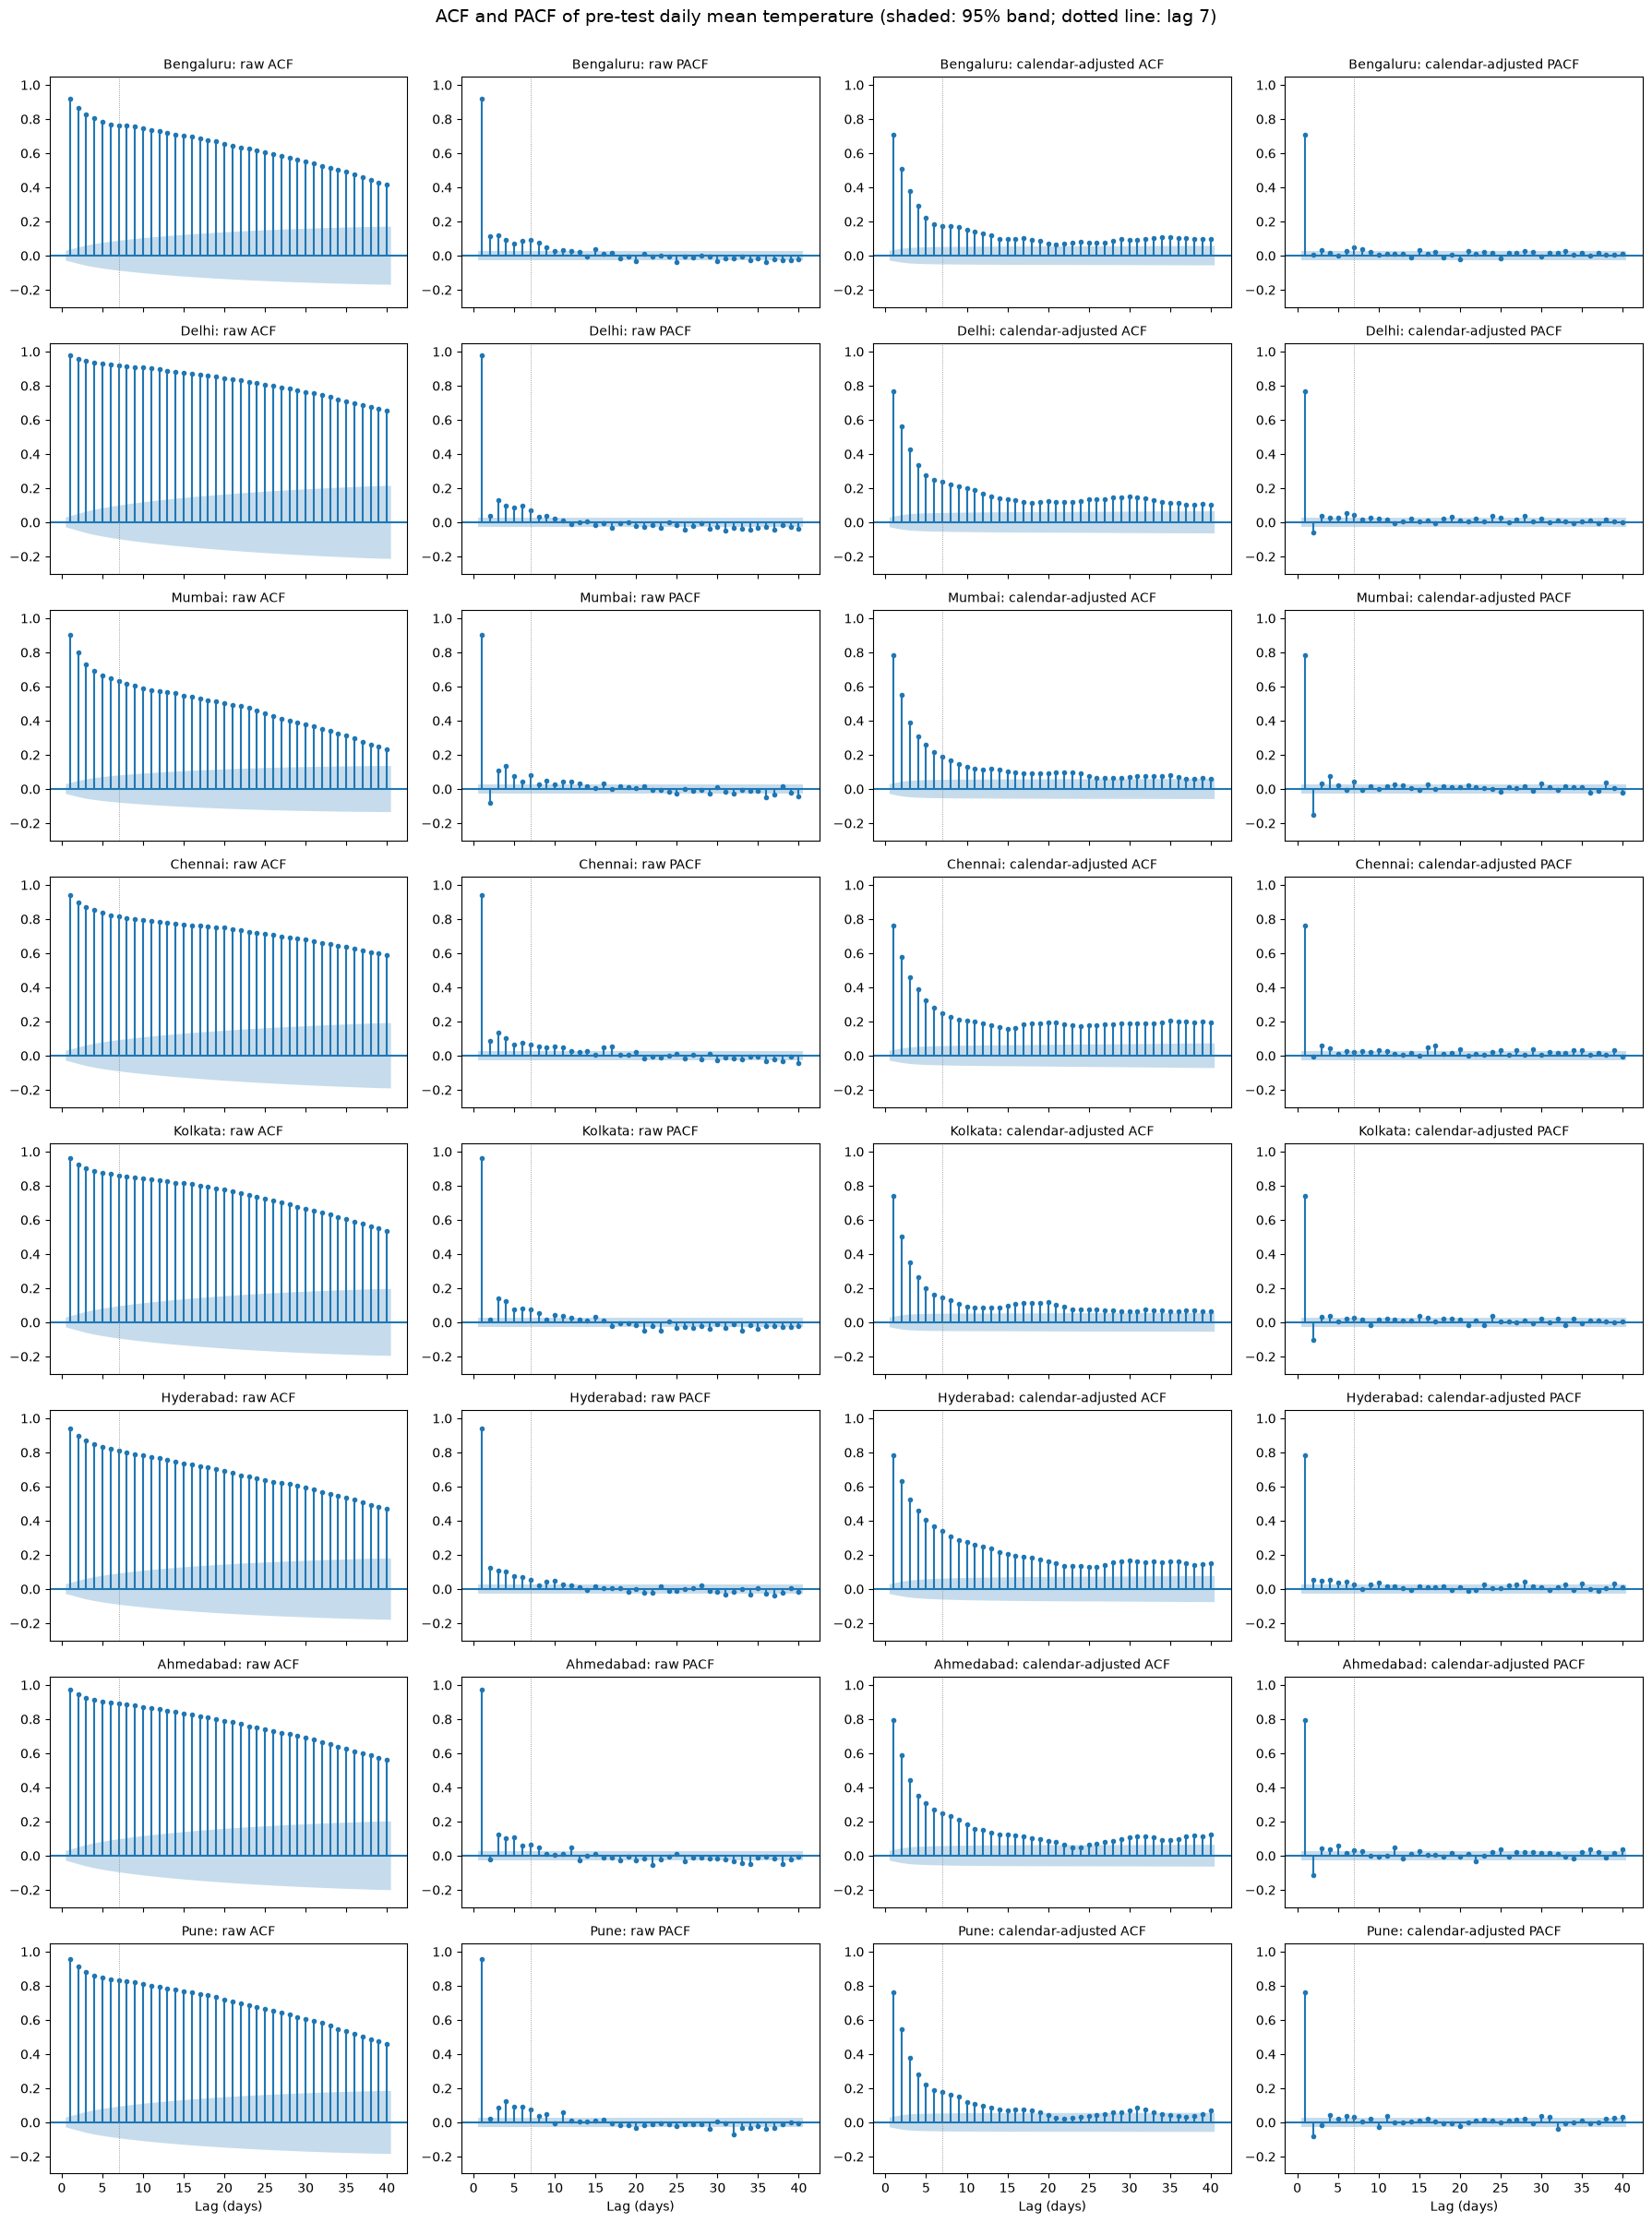
\includegraphics[width=0.94\linewidth]{eight_city_acf_pacf_pretest.png}
\caption{ACF and PACF to lag 40 of the pre-test series (first 85\%) for every station. Left pair: level series, as modelled by ARIMA and SARIMA. Right pair: anomaly after removing the calendar terms of \cref{eq:fourier}, as modelled by ARMAX and SARIMAX. Shaded: 95\% band ($\pm 0.029$). From the executed notebook, Section~4.}
\label{fig:acfpacf}
\end{figure}

\begin{table}[ht]
\centering
\footnotesize
\setlength{\tabcolsep}{3.5pt}
\caption{Correlogram summaries of the pre-test series and the BIC-selected orders. Orders are $(p,d,q)$, with weekly seasonal terms shown as $\times(P,D,Q)_7$ where selected. $\Delta$BIC is the ARIMA BIC minus the ARMAX BIC, i.e.\ the improvement from adding calendar regressors.}
\label{tab:orders}
\resizebox{\linewidth}{!}{%
\begin{tabular}{@{}l r r r r r l l l l r@{}}
\toprule
 & Raw & \multicolumn{4}{c}{Calendar-adjusted} & \multicolumn{4}{c}{BIC-selected order} & \\
\cmidrule(lr){2-2}\cmidrule(lr){3-6}\cmidrule(lr){7-10}
City & PACF$_1$ & PACF$_1$ & PACF$_2$ & PACF$_7$ & ACF$_7$ & ARIMA & SARIMA & ARMAX & SARIMAX & $\Delta$BIC \\
\midrule
\tabfile{tables/r2_orders.tex}
\bottomrule
\end{tabular}}
\end{table}

The level-series correlograms in \cref{fig:acfpacf} repeat what Review 1 found on the full record: a slowly decaying ACF and a PACF dominated by lag 1 (0.90--0.98), with smaller partial autocorrelations that still fall outside the 95\% band up to about lag 7. The calendar-adjusted panels change the picture. Once the annual cycle is removed, the ACF decays geometrically (0.14--0.34 at lag 7), and the PACF cuts off after lag 1 or 2. The adjusted lag-1 PACF lies between 0.71 and 0.79 and the lag-2 value between $-0.15$ and $+0.05$. This is the textbook signature of a low-order autoregression \citep{box2015time}, and it shows that much of the raw partial autocorrelation at lags 2--7 was the unmodelled seasonal cycle rather than short-range dynamics.

The selected orders agree with this reading (\cref{tab:orders}). Every BIC-selected model has $p \in \{1, 2\}$. Where the adjusted PACF has a clear negative lag-2 value, BIC adds a second autoregressive term to the calendar models: Mumbai ($-0.15$), Ahmedabad ($-0.12$; SARIMAX) and Pune ($-0.08$) are all selected with $p = 2$. Bengaluru, whose adjusted PACF is flat after lag 1 ($+0.01$), is an ARMAX(1,0,0). Kolkata and Delhi also have a negative lag-2 value but are fitted as (1,0,1), since one moving-average term reproduces a short negative partial autocorrelation about as well as a second AR term. Chennai, (2,0,2), and Hyderabad, (1,0,2), are the cases where BIC keeps more moving-average terms than the PACF suggests; these are also the two stations whose adjusted ACF decays most slowly (lag 7: 0.25 and 0.34).

Three further patterns stand out.
\begin{itemize}
  \item \textbf{Calendar regressors matter more than ARMA order.} Adding the Fourier terms lowers BIC by 121 (Hyderabad) to 335 (Delhi) points. The raw-series ARIMA models need more terms, (1,0,2) to (2,0,2), because their ARMA polynomials must also mimic the slow seasonal decay.
  \item \textbf{Weekly seasonal terms are marginal.} The adjusted PACF at lag 7 is at most 0.05. BIC keeps a weekly term in 7 of 8 SARIMA and 6 of 8 SARIMAX fits, but the gains are small (13 BIC points for Bengaluru's SARIMA against 307 for its calendar terms), and on the test set SARIMA and ARIMA are almost indistinguishable (\cref{tab:family}). We know of no mechanism that would produce a seven-day temperature cycle at these stations, so we read the weekly terms as fitting chance structure in a long sample rather than as evidence of a weekly effect.
  \item \textbf{AIC and BIC mostly agree.} They choose the same order in 27 of the 32 city--family fits. Where they differ, AIC adds one or two terms, as in Mumbai's ARMAX, where AIC selects (2,0,2) instead of (2,0,0).
\end{itemize}
A lower in-sample BIC does not guarantee a lower test error. For Bengaluru, the BIC-selected ARIMA(1,0,2) has a test RMSE of 0.836\degC, against 0.829\degC{} for the fixed ARIMA(2,0,2) used in Stage A. Across cities the two ARIMA versions differ by at most 0.015\degC{} in RMSE. We report both rather than choose an order on the test set.

\subsection{One-day-ahead accuracy}
\label{sec:accuracy}

\begin{table}[ht]
\centering
\footnotesize
\setlength{\tabcolsep}{3.6pt}
\caption{Best one-step model per city (lowest test RMSE among the 14 Stage B models), cities ordered by that RMSE. Skill follows \cref{eq:skill}. $\bar d$ is the mean absolute-loss difference from persistence (\si{\degreeCelsius}; negative is better) and $p_{\text{Holm}}$ its Holm-adjusted Diebold--Mariano $p$-value; $^{*}$ significant at 5\%.}
\label{tab:best}
\begin{tabular}{@{}l l r r r r r r r r@{}}
\toprule
 & & \multicolumn{2}{c}{Best model (\si{\degreeCelsius})} & \multicolumn{2}{c}{Persistence (\si{\degreeCelsius})} & \multicolumn{2}{c}{Skill (\%)} & & \\
\cmidrule(lr){3-4}\cmidrule(lr){5-6}\cmidrule(lr){7-8}
City & Best model & MAE & RMSE & MAE & RMSE & RMSE & MAE & $\bar d$ & $p_{\text{Holm}}$ \\
\midrule
\tabfile{tables/r2_onestep_best.tex}
\bottomrule
\end{tabular}
\end{table}

\begin{table}[ht]
\centering
\small
\caption{Model averages over the eight cities, each city weighted equally, ordered by mean RMSE. Skill is computed from the mean RMSEs. ``Wins'' counts cities where the model has the lowest RMSE; ``rank'' is the mean of its per-city RMSE rank among 14 models.}
\label{tab:family}
\begin{tabular}{@{}l r r r r r r r@{}}
\toprule
Model & MAE & RMSE & Skill (\%) & MASE & $R^2$ & Wins & Rank \\
\midrule
\tabfile{tables/r2_family.tex}
\bottomrule
\end{tabular}
\end{table}

\begin{figure}[ht]
\centering
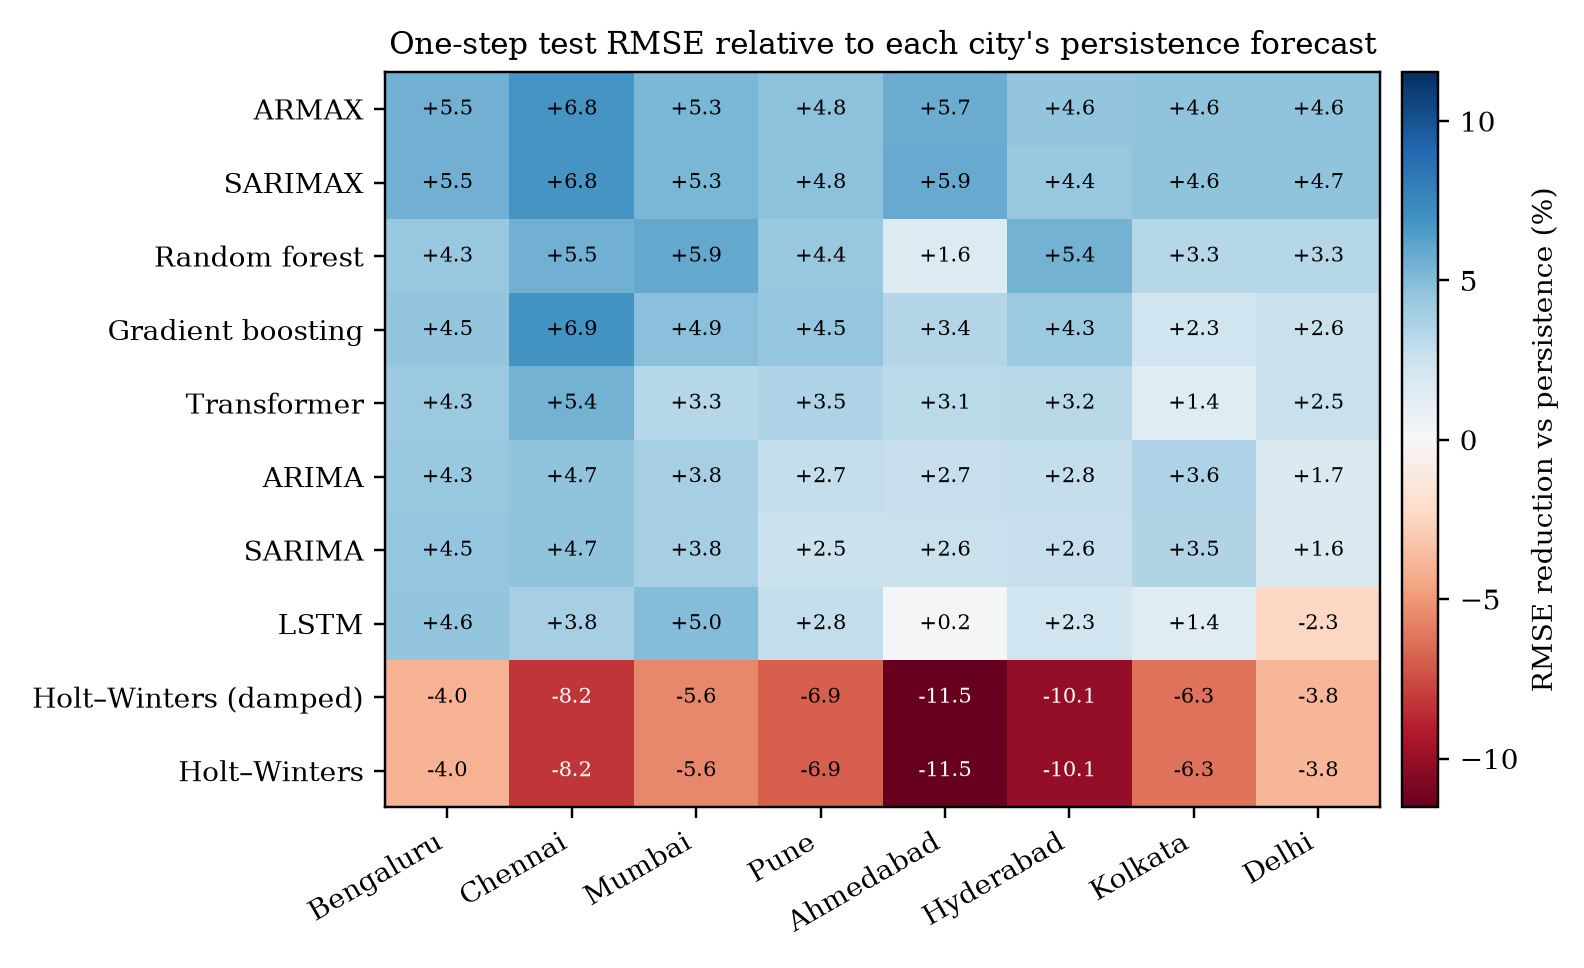
\includegraphics[width=0.9\linewidth]{rmse_skill_heatmap.png}
\caption{Percentage reduction in one-step test RMSE relative to persistence for every non-naive model and city. Cities ordered by best RMSE. Plotted from the saved Stage B metrics (\code{results/rubric\_extension/}).}
\label{fig:heatmap}
\end{figure}

\Cref{tab:best,tab:family} and \cref{fig:heatmap} give the one-step results. Four observations follow.

\emph{No family wins everywhere.} SARIMAX has the lowest RMSE in three cities (Bengaluru, Delhi, Ahmedabad), ARMAX in two (Kolkata, Pune), random forest in two (Mumbai, Hyderabad) and gradient boosting in one (Chennai). Several of these wins are near-ties: SARIMAX leads ARMAX by 0.0003\degC{} at Bengaluru and 0.0001\degC{} at Delhi, gradient boosting leads ARMAX by 0.0005\degC{} at Chennai, and at Pune ARMAX and SARIMAX selected the same (2,0,0) model and tie exactly. ARMAX and SARIMAX share the lowest mean RMSE (1.016\degC) and have the two best mean ranks (1.75 and 2.00). In most cities they produce nearly identical forecasts, because the weekly terms contribute so little.

\emph{The top of the table is crowded.} The seven best methods (ARMAX, SARIMAX, random forest, gradient boosting, Transformer, ARIMA, SARIMA) lie within 0.022\degC{} of each other in mean RMSE, and the LSTM is only 0.035\degC{} behind the leader. Rankings within this group change with the error measure. For Bengaluru, SARIMAX has the lowest RMSE (0.826\degC) but SARIMA the lowest Stage B MAE (0.644\degC), and Stage A's fixed ARIMA(2,0,2) has a lower MAE still (0.638\degC). The ranking of models inside the top group should not be over-read.

\emph{Gains over persistence are real but small.} The best model lowers RMSE by 4.6--6.9\% and MAE by 0.3--6.9\%. In seven of the eight cities the RMSE gain exceeds the MAE gain (Ahmedabad is the exception), which means the models help most on days with large errors. A plausible reason is that persistence is hurt most by abrupt changes, while a model that partly reverts towards the seasonal mean reduces those large misses, which RMSE weights heavily.

\emph{Holt--Winters is worse than persistence in every city}, by 3.8--11.5\% in RMSE, and the Diebold--Mariano test confirms the deficit after Holm correction in all eight cities. The damped and undamped variants are indistinguishable. A plausible explanation is the seasonal period: with $m = 365$, each seasonal index in \cref{eq:hw} is updated once a year from a single day's observation, so the seasonal component inherits much of a previous year's day-level noise. The fitted smoothing parameters were not saved, so we cannot confirm this mechanism from the outputs. Seasonal naive forecasts and the climatological mean are 2.0--3.4 times worse than persistence in mean RMSE. The seasonal pattern alone is a poor next-day forecast; the information is in yesterday's value.

\subsection{Statistical significance of the gains}
\label{sec:dm}

The Diebold--Mariano results in \cref{tab:best} temper the accuracy table. The selected model has lower mean absolute loss than persistence in all eight cities, but the reductions are 0.003--0.054\degC{} per day. After Holm correction they are significant only in Ahmedabad (SARIMAX, $\bar d = -0.054$\degC, $p_{\text{Holm}} = 0.0001$), Delhi (SARIMAX, $-0.047$\degC, $p = 0.006$) and Chennai (gradient boosting, $-0.028$\degC, $p = 0.011$). In the other five cities the test cannot distinguish the best model from persistence. This does not show that the two are equivalent, only that 822 days are not enough to detect a difference of this size.

Two points qualify the comparison. First, the test is on absolute loss, whereas the models are ranked by RMSE. A model can rank first by RMSE because it avoids a few large errors while gaining nothing on typical days, which is what happens for Bengaluru. Its SARIMAX has the best RMSE but an insignificant absolute-loss difference ($p_{\text{Holm}} = 1$), while SARIMA has the largest absolute-loss reduction ($\bar d = -0.024$\degC, unadjusted $p = 0.009$), which loses significance after correction ($p_{\text{Holm}} = 0.068$). Second, in Delhi and Ahmedabad only ARMAX and SARIMAX beat persistence significantly, whereas in Chennai six models do: gradient boosting, ARMAX, SARIMAX, ARIMA, SARIMA and the LSTM.

For the neural models the evidence on H0 is clear. The Transformer's absolute-loss improvement over persistence is not significant in any city, and the LSTM's only in Chennai ($p_{\text{Holm}} = 0.040$). The LSTM is significantly \emph{worse} than persistence before correction in Delhi (unadjusted $p = 0.043$), though not after. The original single-station report stated that H0 was rejected because the LSTM and Transformer had a lower test MAE than persistence; with a paired test that conclusion does not hold. At one day ahead we cannot reject H0 for the sequence models in seven of the eight cities.

\subsection{Reconciling Stage A with Stage B}
\label{sec:reconcile}

\begin{table}[ht]
\centering
\small
\caption{Stage A one-step test MAE (\si{\degreeCelsius}) for persistence, the fixed ARIMA(2,0,2) and the two neural models, with the neural models' MAE skill relative to persistence (\%).}
\label{tab:stageA}
\begin{tabular}{@{}l r r r r r r@{}}
\toprule
City & Persistence & ARIMA(2,0,2) & LSTM & Transformer & LSTM skill & Transformer skill \\
\midrule
\tabfile{tables/r2_stageA.tex}
\bottomrule
\end{tabular}
\end{table}

Stage A, with a smaller candidate set, named the Transformer as the best one-step model in five cities (\code{report/city\_comparison.md}). \Cref{tab:stageA} shows why this label should not be taken as a finding. The Transformer's MAE advantage over persistence in those cities is at most 2.7\%, and in Kolkata both neural models are worse than persistence. When the fixed ARIMA(2,0,2) from Stage A is pooled with the 14 Stage B models, the overall RMSE winner is the Stage B winner in every city. The neural models never win a city in Stage B.

\subsection{Multi-horizon forecasts}
\label{sec:horizon}

\begin{table}[ht]
\centering
\footnotesize
\setlength{\tabcolsep}{3.8pt}
\caption{Stage A direct multi-horizon results over 792 test origins. Left: Transformer MAE (\si{\degreeCelsius}) at selected leads. Middle: MAE averaged over leads 1, 7, 14, 21 and 30 days. Right: Transformer reduction in that average relative to persistence and to the annual seasonal naive forecast (\%).}
\label{tab:horizon}
\begin{tabular}{@{}l rrrrr rrrr rr@{}}
\toprule
 & \multicolumn{5}{c}{Transformer MAE at lead (days)} & \multicolumn{4}{c}{Mean over leads} & \multicolumn{2}{c}{Transformer skill vs} \\
\cmidrule(lr){2-6}\cmidrule(lr){7-10}\cmidrule(l){11-12}
City & 1 & 7 & 14 & 21 & 30 & Pers. & S.\ naive & LSTM & Transf. & Pers. & S.\ naive \\
\midrule
\tabfile{tables/r2_horizon.tex}
\bottomrule
\end{tabular}
\end{table}

\begin{figure}[ht]
\centering
\begin{subfigure}{0.49\linewidth}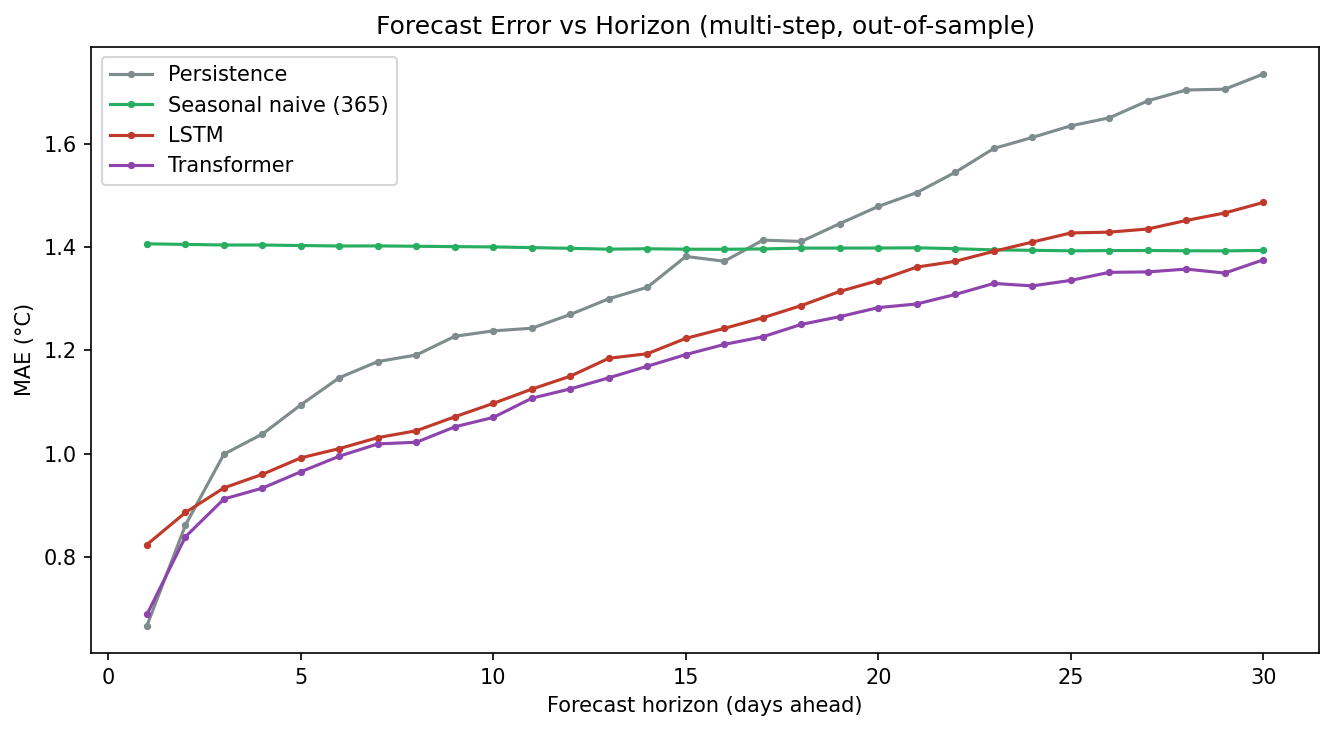
\includegraphics[width=\linewidth]{bengaluru_error_vs_horizon.png}\caption{Bengaluru, all leads 1--30}\end{subfigure}\hfill
\begin{subfigure}{0.49\linewidth}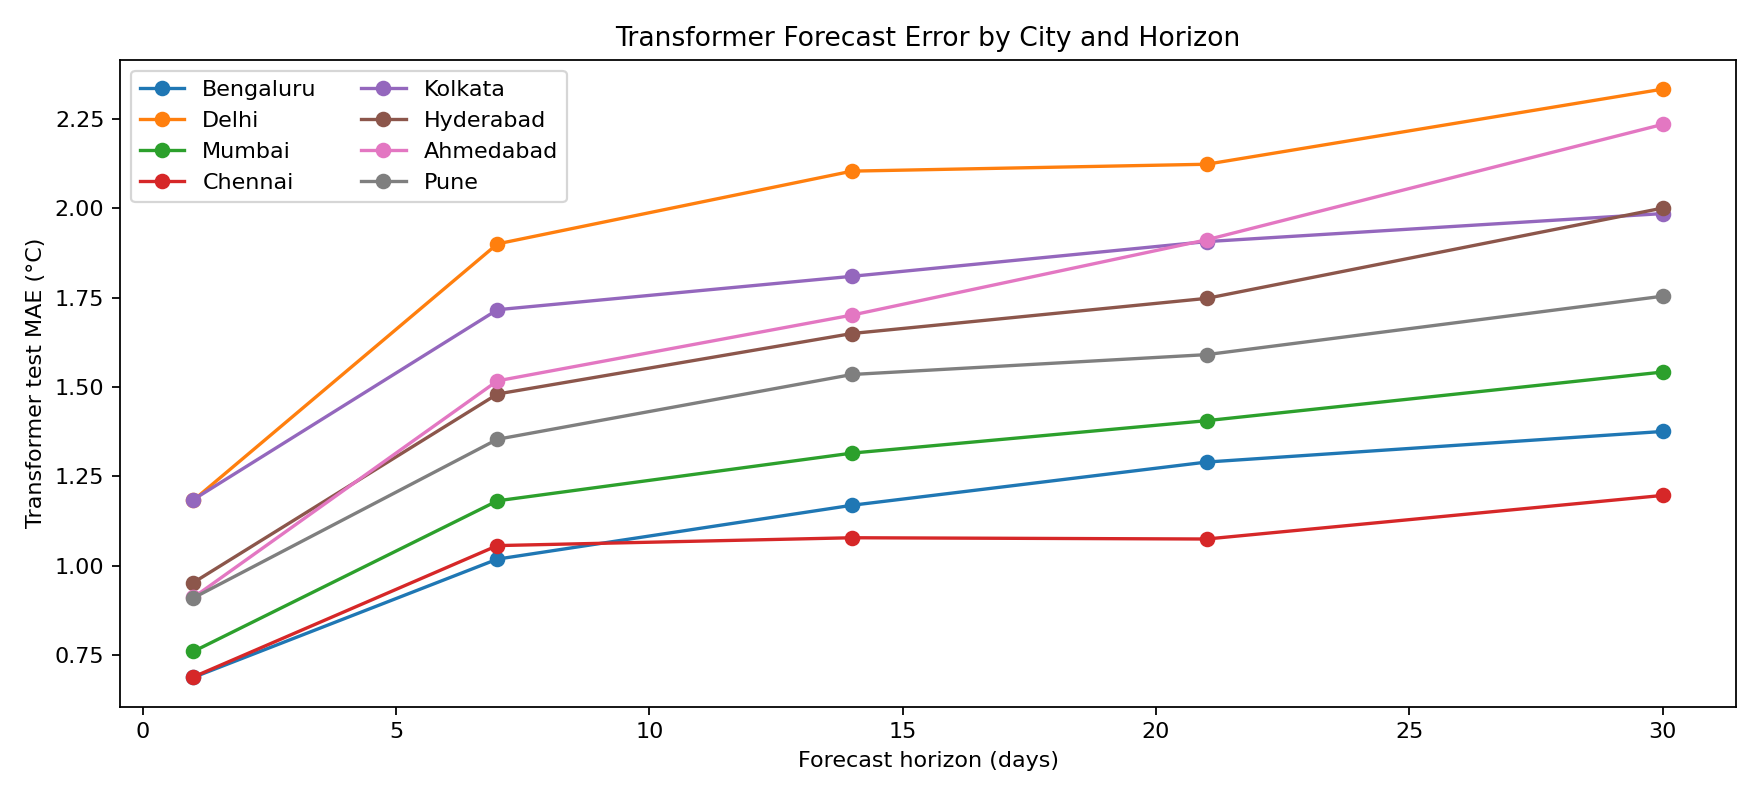
\includegraphics[width=\linewidth]{transformer_horizon_mae.png}\caption{Transformer, all cities, selected leads}\end{subfigure}
\caption{Test MAE as a function of forecast lead.}
\label{fig:horizon}
\end{figure}

The multi-horizon experiment (\cref{tab:horizon}, \cref{fig:horizon}) behaves as H2 predicts. Persistence is the best method at one day but degrades fastest: at Bengaluru its MAE rises from 0.67\degC{} at one day to 1.74\degC{} at 30 days, and at Delhi from 1.05\degC{} to 4.29\degC. The annual seasonal naive forecast is flat across leads because it ignores recent weather entirely. The Transformer lies between the two, close to persistence at short leads and close to or below the seasonal naive forecast at long ones. Averaged over the five reported leads it is 11.8--30.6\% better than persistence and 16.0--27.0\% better than the seasonal naive forecast, and it beats the LSTM at every city. The gain over persistence is largest in Delhi, where the annual swing is largest and a 30-day-old temperature is therefore most out of date.

Three details limit this result. First, at one day the direct multi-output models are worse than persistence in every city (for example, Transformer 0.69\degC{} against persistence 0.67\degC{} at Bengaluru), because a network trained for all 30 leads at once spends capacity on the long ones. Second, the Transformer does not dominate the seasonal naive forecast everywhere. At Ahmedabad its 30-day MAE (2.23\degC) is worse than the seasonal naive forecast's (2.04\degC), and at four other stations (Bengaluru, Chennai, Mumbai, Hyderabad) the two are within 0.04\degC{} at 30 days. Third, no ARIMA-family or tree model was run at these horizons, and no significance test was applied, so the multi-horizon comparison covers only the neural models and the two naive references, and its gains are measured, not tested.

\subsection{Residual diagnostics}
\label{sec:residuals}

\begin{table}[ht]
\centering
\footnotesize
\setlength{\tabcolsep}{2.9pt}
\caption{Test-period residual diagnostics ($e_t = y_t - \hat y_t$, $N = 822$) for each city's selected model. $t$ is the bias $t$-statistic. LB$_{10}$ and LB$_{30}$: Ljung--Box $p$-values. JB: Jarque--Bera statistic (all $p < 10^{-10}$). Tails: percentage of centred residuals below $-1.96$\,SD and above $+1.96$\,SD (2.5\% each under normality). Last column: number of the 14 models in that city whose residuals fail LB$_{30}$ at 5\%.}
\label{tab:residuals}
\begin{tabular}{@{}l l r r r r r r r r r c r@{}}
\toprule
City & Model & Bias & $t$ & SD & DW & LB$_{10}$ & LB$_{30}$ & JB & Skew & Ex.\ kurt. & Tails (\%) & Fail \\
\midrule
\tabfile{tables/r2_residuals.tex}
\bottomrule
\end{tabular}
\end{table}

\begin{figure}[p]
\centering
\begin{subfigure}{0.80\linewidth}\centering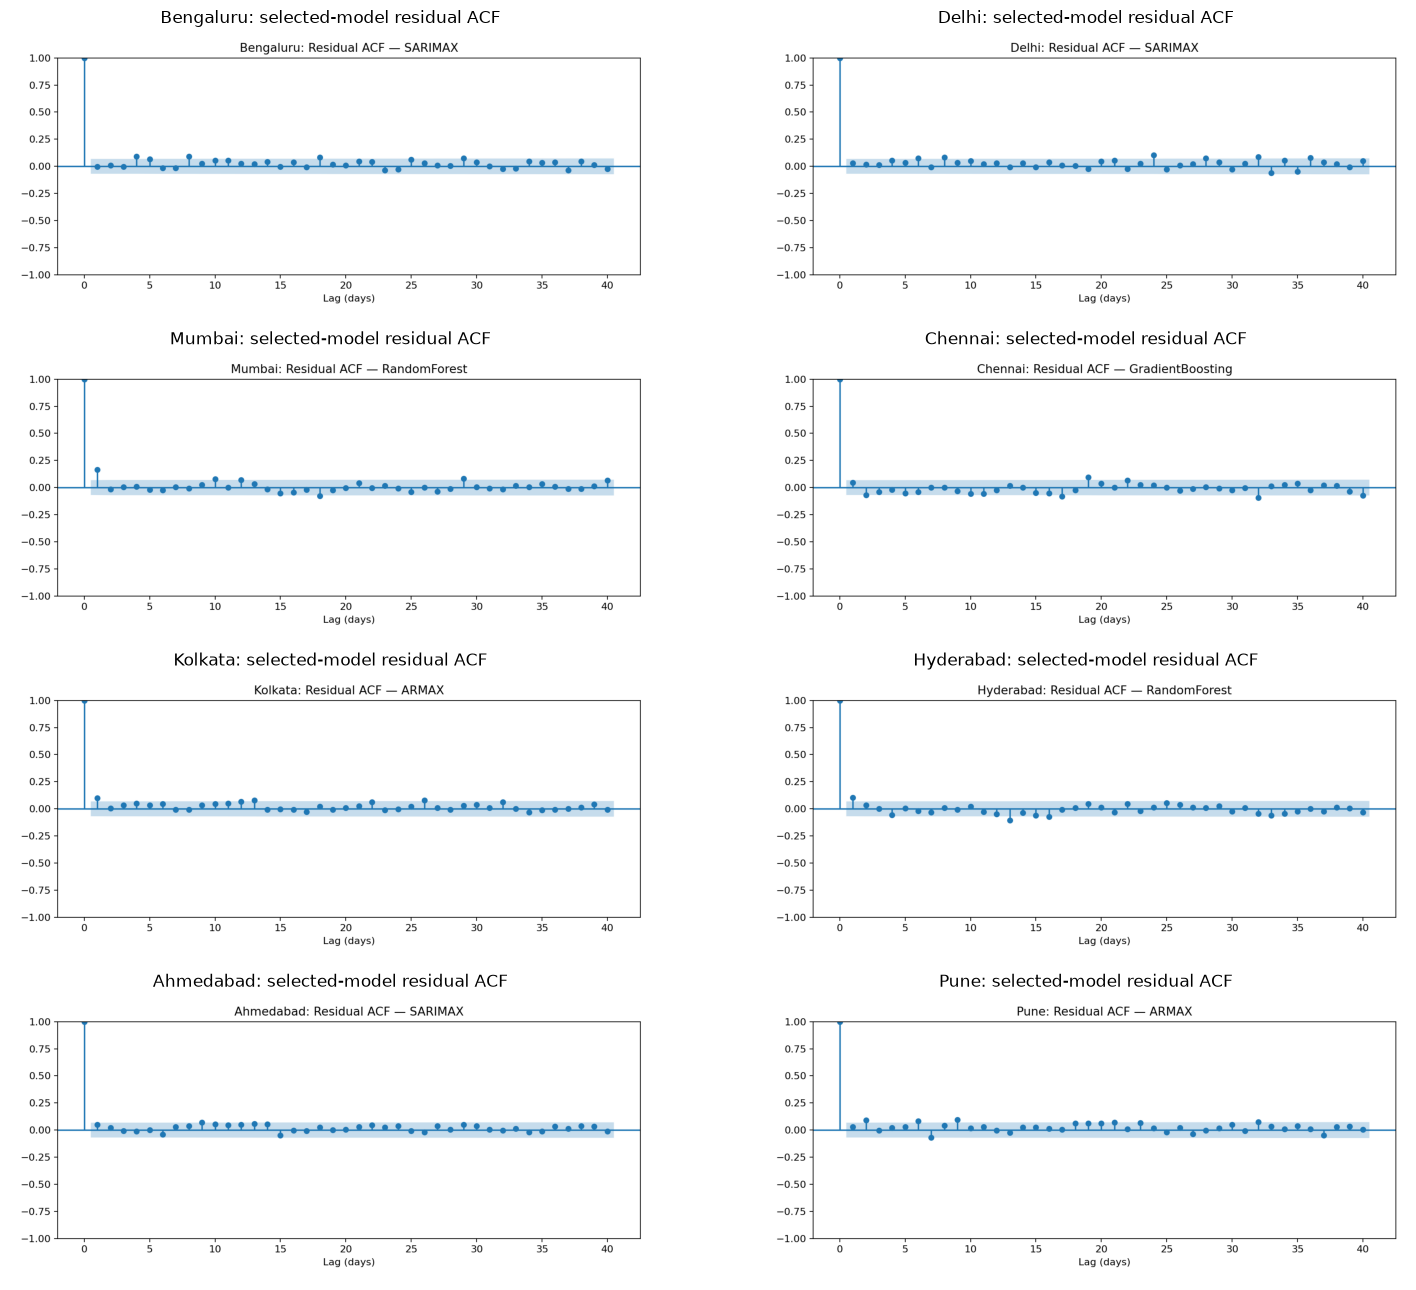
\includegraphics[width=\linewidth]{eight_city_residual_acf.png}\caption{Residual ACF of each city's selected model, lags 1--40}\end{subfigure}\\[6pt]
\begin{subfigure}{0.80\linewidth}\centering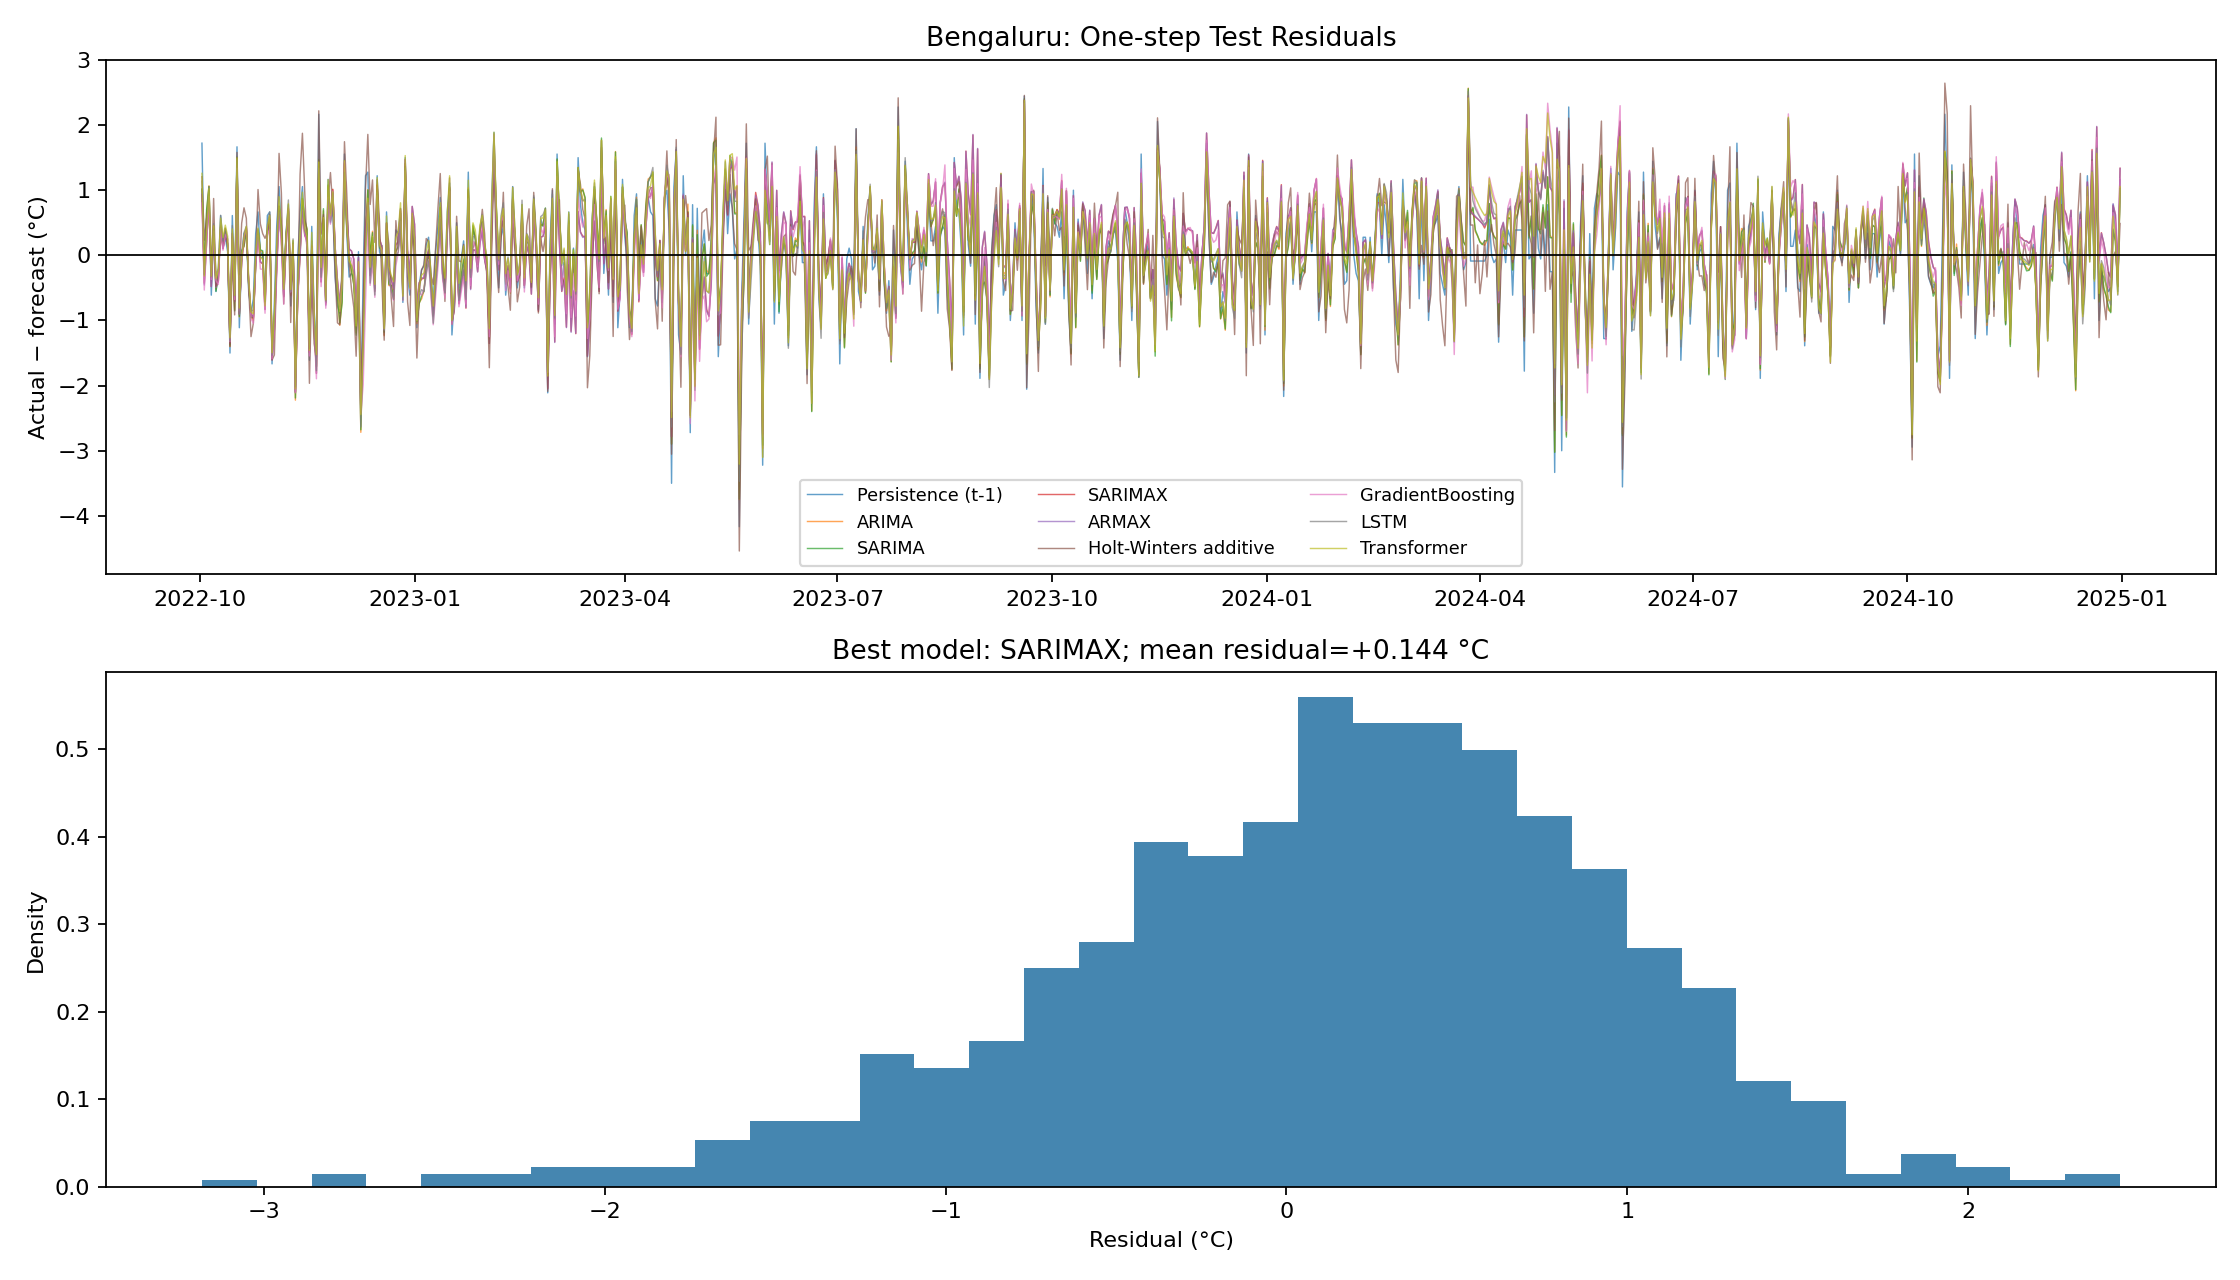
\includegraphics[width=\linewidth]{bengaluru_residual_diagnostics.png}\caption{Bengaluru: residuals over time for several models (top) and SARIMAX residual histogram (bottom)}\end{subfigure}
\caption{Residual diagnostics on the 822 test days.}
\label{fig:residuals}
\end{figure}

\paragraph{Bias.} Mean residuals range from $-0.11$ to $+0.21$\degC, small next to residual standard deviations of 0.81--1.33\degC. Five have $|t| > 1.96$, but two stand out: Bengaluru's SARIMAX ($+0.14$\degC, $t = 5.1$) and Kolkata's ARMAX ($+0.21$\degC, $t = 4.9$). Delhi, Mumbai and Ahmedabad have biases of about 0.07--0.11\degC{} ($|t|$ 2.2--2.4). Both under-forecast the test period. In the same cities the plain ARIMA, which has no calendar terms, is almost unbiased ($+0.015$ and $-0.023$\degC). This pattern is consistent with the 2022--2024 test period being slightly warmer than the 2010--2022 seasonal mean encoded by the calendar terms. ARIMA, whose forecasts lean more heavily on the latest observations, follows such a shift, while the calendar models pull towards the older seasonal mean. Re-estimating the intercept on recent data would be a simple remedy, though we have not tested it.

\paragraph{Serial dependence.} At lag 30, the Ljung--Box test rejects white-noise residuals at the 5\% level in five cities: Mumbai ($p = 0.005$), Pune (0.006), Bengaluru (0.020), Hyderabad (0.037) and Delhi (0.048). With eight cities tested, a Bonferroni threshold of $0.05/8 = 0.006$ leaves only Mumbai and Pune. The remaining dependence is small: the largest residual autocorrelation over lags 1--30 is 0.07--0.16, against a 95\% band of $\pm 0.068$. The clearest exception is Mumbai's random forest, with lag-1 residual autocorrelation 0.16 (Durbin--Watson 1.66). A tree model has no moving-average error term, so day-to-day carry-over in its own errors goes unmodelled. Residual autocorrelation is not specific to the selected models: in each city, 7--13 of the 14 models fail the lag-30 test. That points to weather dynamics that no univariate model here captures, rather than to a defect of one model.

\paragraph{Distribution.} Normality is rejected decisively everywhere (Jarque--Bera statistics 49--532). The departure has the same shape in every city: negative skewness ($-0.14$ to $-0.76$) and excess kurtosis (0.66--3.70). Large errors are mostly over-forecasts, days that turned out much colder than predicted, with 2.7--4.3\% of residuals below $-1.96$\,SD but only 1.3--2.7\% above $+1.96$\,SD. Sudden cooling from rain or from cold-air outbreaks would produce this pattern, and a univariate model cannot anticipate either. Point metrics and the HAC-based Diebold--Mariano test do not assume normal or independent errors, so the rankings above stand. Symmetric Gaussian prediction intervals, however, would be miscalibrated on the cold side; empirical-quantile or bootstrap intervals would be needed for uncertainty statements.

\paragraph{Failure cases.} Stage A recorded, for each city, the ten test days with the largest one-step errors of the LSTM and of the Transformer. Between 6 (Kolkata) and 10 (Bengaluru, Chennai, Hyderabad) of these ten dates are shared by the two networks, and none of them falls on an interpolated day in any city (the pipeline checked the LSTM's ten dates; we rechecked the Transformer's). At Bengaluru the shared dates include 2023-04-21, 2023-05-20, 2024-05-08 and 2024-06-01, in the pre-monsoon and monsoon-onset period (\cref{fig:spikes}). Two architecturally different models failing on the same days suggests the errors come from the weather itself, from abrupt changes that are not foreshadowed in the preceding 30 days of temperature, rather than from a data artefact or a weakness of one architecture.

\begin{figure}[ht]
\centering
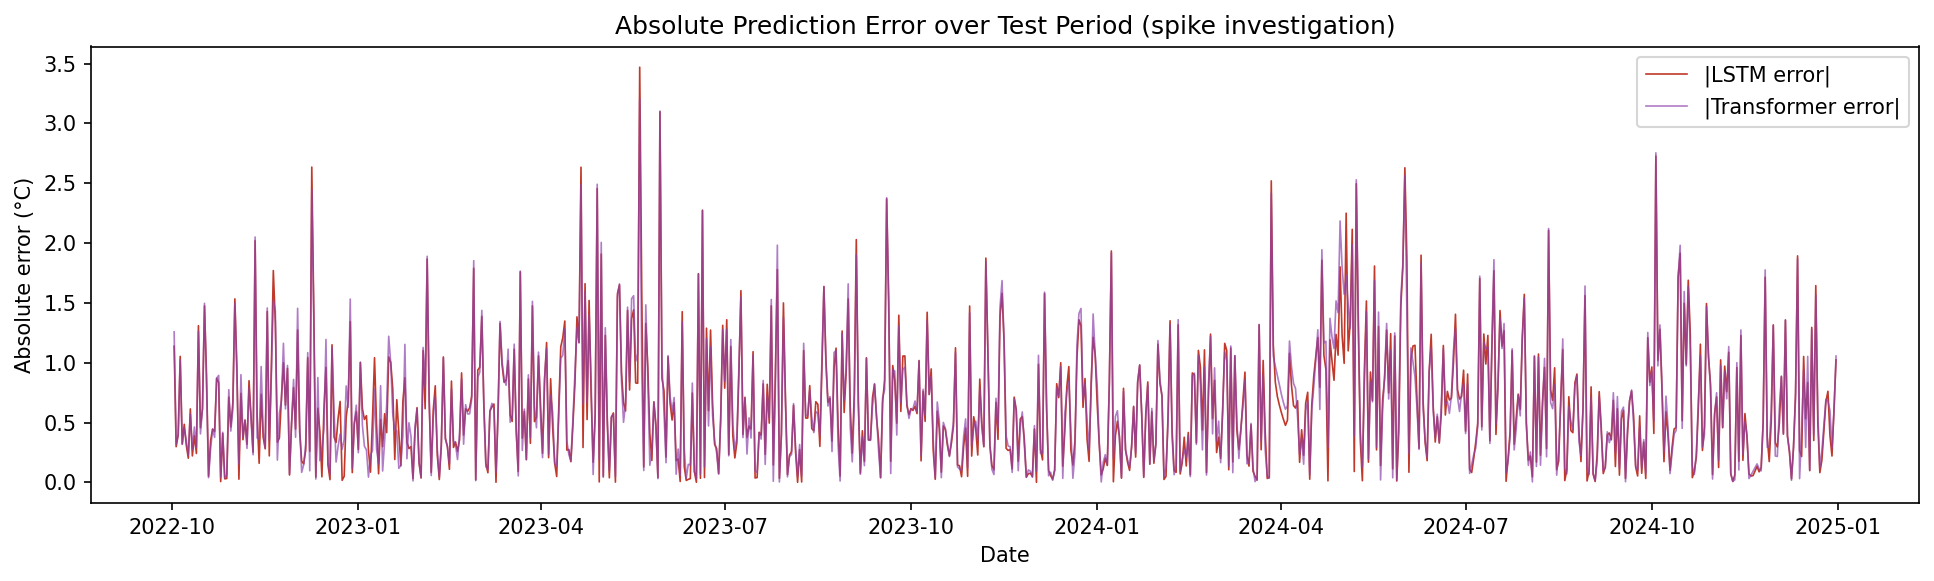
\includegraphics[width=0.92\linewidth]{bengaluru_error_spikes.png}
\caption{Absolute one-step test errors of the Stage A LSTM and Transformer at Bengaluru. The large spikes coincide for the two models.}
\label{fig:spikes}
\end{figure}

\section{Discussion}
\label{sec:discussion}

\subsection{Why cities differ}

\begin{figure}[ht]
\centering
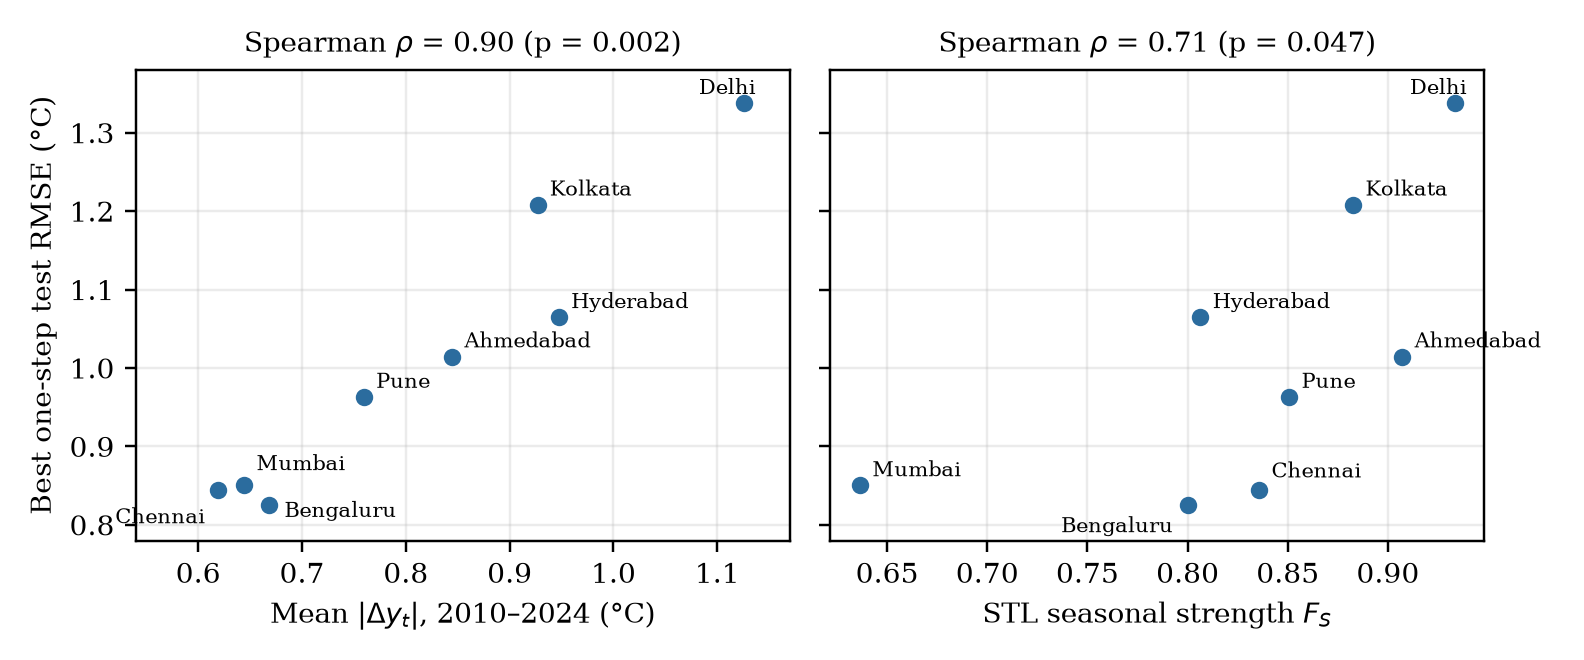
\includegraphics[width=0.92\linewidth]{difficulty_vs_variability.png}
\caption{Best one-step test RMSE against the 2010--2024 mean absolute daily change (left) and the STL seasonal strength (right), one point per station.}
\label{fig:difficulty}
\end{figure}

The best attainable one-step RMSE differs by a factor of 1.6 between cities (\cref{tab:best}), far more than the spread between the top models within any city. \Cref{fig:difficulty} shows that the city ordering follows the mean absolute daily change measured in Review 1 (Spearman $\rho = 0.90$, $p = 0.002$) more closely than seasonal strength ($\rho = 0.71$, $p = 0.047$). The exceptions are informative. Mumbai has the weakest annual cycle ($F_S = 0.64$) yet is among the easiest stations, and Chennai's cycle is stronger than Hyderabad's although Chennai is much easier to forecast. The annual cycle describes how far the seasonal mean moves over a year, whereas one-step error depends on how far temperature moves overnight, and the two are different properties. Persistence MAE follows almost the same city ordering (0.64\degC{} at Mumbai to 1.05\degC{} at Delhi). The differences therefore reflect the stations' climates rather than how well each model suited them.

This is a correlation across eight stations, measured on one test period. It supports H2 descriptively but does not establish why some stations have larger daily changes. Plausible explanations include the moderating effect of the sea at Mumbai and Chennai and the larger synoptic disturbances that reach northern inland stations such as Delhi, but we have not tested them.

\subsection{Statistical versus deep-learning models}

At one day ahead the simplest adequate model wins. The calendar-adjusted correlograms show that, once the annual mean is removed, temperature behaves like an AR(1) or AR(2) process. ARMAX represents that structure exactly with a few parameters and is estimated on all 4{,}657 pre-test days. The LSTM and Transformer must learn the same near-linear relation from 3{,}805 windows, and they receive no calendar information. They come close (Transformer mean RMSE 1.037\degC{} against 1.016\degC) but do not surpass it. The tree ensembles, which do get the calendar terms and the larger training set, close most of the gap. These comparisons mix three differences (model class, calendar features and amount of training data), so they cannot isolate the contribution of the architecture.

The picture changes with lead time. At 7--30 days the Transformer clearly beats persistence and, in most cities, the seasonal naive forecast. A direct multi-output network can learn how quickly to move from recent anomalies towards the seasonal mean as lead time grows, which neither naive method does. Whether a calendar-aware ARMAX would do as well at those leads was not tested.

\subsection{Do the results support the hypotheses?}

\begin{itemize}
  \item \textbf{H1} is supported in its first part and partly in its second. Every learned model beats the mean and seasonal-naive baselines by a wide margin, and the best model in every city has lower RMSE and MAE than persistence. The improvement is statistically significant in only three cities.
  \item \textbf{H0} cannot be rejected for the LSTM and Transformer at one day ahead in seven of eight cities. The original single-station claim to the contrary rested on point estimates without a paired test.
  \item \textbf{H2} is supported descriptively on both counts: city difficulty follows daily variability ($\rho = 0.90$), and the Transformer's gain over persistence grows from at most 2.7\% at one day (\cref{tab:stageA}) to 11.8--30.6\% averaged over 1--30 days.
\end{itemize}
The data do not support a claim that any one family is generally superior. The leading families differ by hundredths of a degree, rankings depend on the error measure, and they come from one 27-month test period.

\section{Limitations and threats to validity}
\label{sec:limits}

\begin{itemize}
  \item \textbf{Single holdout.} All results come from one chronological split. A rolling-origin evaluation would show whether the rankings are stable across years and seasons.
  \item \textbf{Unequal training data and inputs.} ARIMA-family, Holt--Winters and tree models are fitted on 85\% of the record; the neural models on 70\%, with the remaining 15\% used for early stopping. Only ARMAX, SARIMAX and the tree models receive calendar features. The comparison between families is therefore a comparison of complete modelling pipelines, not of model classes alone.
  \item \textbf{Untuned models.} Tree and neural hyperparameters were fixed in advance and are small by design; tuning on the validation segment could change the order within the top group.
  \item \textbf{Loss mismatch.} Models are ranked by RMSE but tested by absolute loss. A squared-loss Diebold--Mariano test could give different significance results.
  \item \textbf{Multiple testing across cities.} Holm correction is applied within each city, not across the 104 city--model tests.
  \item \textbf{Multi-horizon boundary overlap.} In the direct multi-horizon experiment, a window whose origin lies in the validation segment has targets up to 30 days ahead. The last validation windows therefore include the first 30 test days as targets, and those days influence when training stops. The effect is confined to choosing an epoch, but strictly the first 30 test days are not unseen for these models.
  \item \textbf{Calendar-term phase.} The ARMAX/SARIMAX weekly regressors are two days out of phase between the fitting and test periods (\cref{sec:models}); the effect was not measured.
  \item \textbf{Interpolated inputs.} Up to 1.2\% of each series, and 9--18 of the 822 test days per city, were filled by interpolation that uses the following observation. No large forecast error fell on such a day, and the effect is shared by all models.
  \item \textbf{One station per city and univariate inputs.} Results describe airport or observatory sites, not whole cities. No humidity, pressure, wind or rainfall predictors were used, although the residual analysis suggests that such predictors are where the remaining predictability lies.
\end{itemize}

\section{Conclusions and future work}
\label{sec:conclusion}

For next-day temperature at these eight stations, ARMA models with Fourier calendar regressors were the most consistent choice. Their BIC-selected orders contain one or two autoregressive terms, as the calendar-adjusted PACF predicts, and they had the lowest RMSE in five cities and the lowest mean RMSE overall. Tree ensembles were as good in some cities. The LSTM and Transformer did not add value at one day: their gains over persistence were small and, with one exception, not significant. At leads of one to four weeks, the direct multi-output Transformer reduced mean error by 12--31\% relative to persistence and by 16--27\% relative to the seasonal naive forecast, the clearest case for a learned model in this study, though the gains were not significance-tested.

The largest differences in this study were between cities, not between models. Delhi's best one-step RMSE is 1.6 times Bengaluru's, and the ordering of cities follows how much temperature changes from one day to the next. For a forecaster, choosing the location matters more than choosing a model among the top group.

The residuals indicate where to go next. Cold-side heavy tails and residual autocorrelation shared by most models point to weather that a univariate temperature history cannot anticipate. The most promising extensions are therefore exogenous predictors (humidity, pressure, wind, rainfall) and a rolling-origin evaluation, together with ARMAX and tree models at multi-day leads, squared-loss significance tests, and empirical prediction intervals that reflect the asymmetric error distribution.

\section{Individual contributions}
\label{sec:contrib}

The team divided the work equally. The table reproduces the contribution record in the project notebook (Section~10) and \code{report/remaining\_rubric\_analysis.md}.

\begin{table}[ht]
\centering
\small
\caption{Contribution record (one third each).}
\label{tab:contrib}
\begin{tabularx}{\linewidth}{@{}l L L@{}}
\toprule
Member & Contribution & Evidence \\
\midrule
Kushal Yalamanchi & Data acquisition and cleaning for all eight stations; visualisation; trend and seasonal decomposition; ADF/KPSS tests; ACF/PACF analysis; review of residual diagnostics & \nolinkurl{src/download_data.py}, \nolinkurl{src/preprocessing.py}, \nolinkurl{src/cities.py}, \nolinkurl{src/statistical_analysis.py}; notebook Sections 2--4 \\
\addlinespace
Kushaal K N & Baselines; order selection for ARIMA, SARIMA, ARMAX and SARIMAX; Holt--Winters; residual analysis (Ljung--Box, Jarque--Bera, Durbin--Watson); review of ML/DL models & \nolinkurl{src/rubric_extension.py}; notebook Sections 5--6 and 8 \\
\addlinespace
Dhrusheek & LSTM and Transformer and the multi-horizon experiment; random forest and gradient boosting; cross-city comparison and Diebold--Mariano tests; research conclusion; report and notebook assembly & \nolinkurl{src/models.py}, \nolinkurl{src/run_all_cities.py}, \nolinkurl{src/run_analysis.py}, \nolinkurl{src/build_notebook.py}; \nolinkurl{report/}; notebook Sections 7 and 9 \\
\bottomrule
\end{tabularx}
\end{table}

\bibliographystyle{plainnat}
\bibliography{references}

\clearpage
\appendix

\section{Full one-step results}
\label{app:full}

\begin{table}[ht]
\centering
\footnotesize
\setlength{\tabcolsep}{4pt}
\caption{One-step test RMSE (\si{\degreeCelsius}) for every model and city. Bold: lowest in the column.}
\label{tab:full_rmse}
\begin{tabular}{@{}l rrrrrrrr@{}}
\toprule
Model & Bengaluru & Delhi & Mumbai & Chennai & Kolkata & Hyderabad & Ahmedabad & Pune \\
\midrule
\tabfile{tables/r2_full_rmse.tex}
\bottomrule
\end{tabular}
\end{table}

\begin{table}[ht]
\centering
\footnotesize
\setlength{\tabcolsep}{4pt}
\caption{One-step test MAE (\si{\degreeCelsius}) for every model and city. Bold: lowest in the column.}
\label{tab:full_mae}
\begin{tabular}{@{}l rrrrrrrr@{}}
\toprule
Model & Bengaluru & Delhi & Mumbai & Chennai & Kolkata & Hyderabad & Ahmedabad & Pune \\
\midrule
\tabfile{tables/r2_full_mae.tex}
\bottomrule
\end{tabular}
\end{table}

\begin{figure}[ht]
\centering
\begin{subfigure}{0.48\linewidth}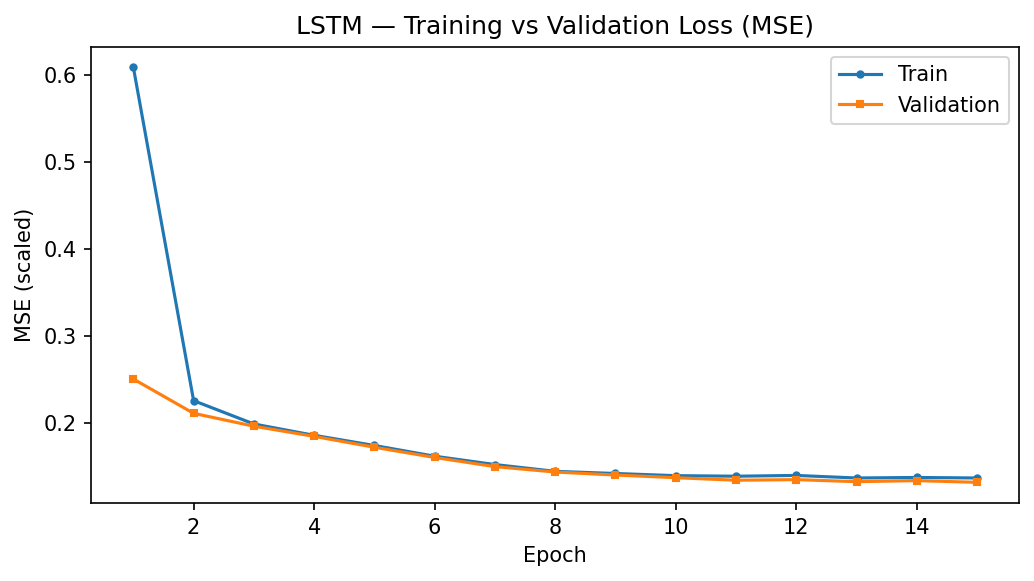
\includegraphics[width=\linewidth]{bengaluru_lstm_loss.png}\caption{LSTM}\end{subfigure}\hfill
\begin{subfigure}{0.48\linewidth}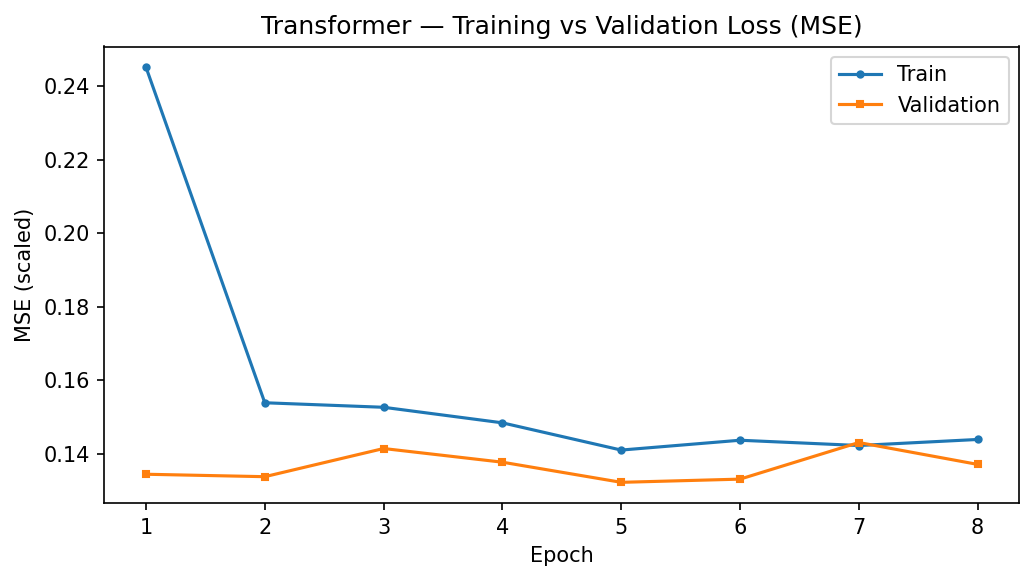
\includegraphics[width=\linewidth]{bengaluru_transformer_loss.png}\caption{Transformer}\end{subfigure}
\caption{Training and validation loss (MSE on standardised data) of the one-step neural models at Bengaluru. Training stops when validation loss has not improved for three epochs; validation loss does not rise sharply, so there is no sign of strong over-fitting within the epoch budget.}
\label{fig:loss}
\end{figure}

\section{Rubric coverage and reproduction}
\label{app:rubric}

The Review 2 components and their marks are taken from the rubric checklist in the project notebook (Section~11).

\begin{center}
\small
\begin{tabular}{@{}l r l@{}}
\toprule
Component & Marks & Where addressed \\
\midrule
ARIMA/SARIMA/ARMAX/SARIMAX and order selection & 3 & \cref{sec:models}, \cref{sec:orders} \\
Holt--Winters & 3 & \cref{sec:models}, \cref{sec:accuracy} \\
Machine-learning and deep-learning models & 3 & \cref{sec:models}, \cref{sec:accuracy,sec:horizon} \\
Baseline forecasts & 2 & \cref{sec:models}, \cref{tab:family} \\
Forecast accuracy & 2 & \cref{sec:accuracy}, \cref{app:full} \\
Model comparison & 2 & \cref{sec:accuracy,sec:dm,sec:reconcile} \\
Residual analysis & 3 & \cref{sec:residuals} \\
Research conclusion & 2 & \cref{sec:discussion,sec:conclusion} \\
Individual contribution & 5 & \cref{sec:contrib} \\
\midrule
Total & 25 & \\
\bottomrule
\end{tabular}
\end{center}

\noindent All numbers were generated from the saved outputs in the repository \url{https://github.com/dhrusheek/noaa-weather-time-series-case-study} by \nolinkurl{submission/scripts/build_assets.py}. To regenerate the outputs themselves, run \code{python} \nolinkurl{src/download_data.py}, then \code{python} \nolinkurl{src/run_all_cities.py} (Stage A) and \code{python} \nolinkurl{src/rubric_extension.py} (Stage B). The executed walkthrough is \nolinkurl{notebooks/eight_city_weather_forecasting_comparison.ipynb}.

\end{document}
